%%%%%%%%%%%%%%%%%%%%%%%%%%%%%%%%%%%%%%%%%%%%%%%%%%%%%%%%%%%%%%%%%%%%%%%%%%%%%%%%
\chapter{ПРОЕКТИРОВАНИЕ И РЕАЛИЗАЦИЯ ПРОГРАММНОГО ОБЕСПЕЧЕНИЯ}
%%%%%%%%%%%%%%%%%%%%%%%%%%%%%%%%%%%%%%%%%%%%%%%%%%%%%%%%%%%%%%%%%%%%%%%%%%%%%%%%

%%%%%%%%%%%%%%%%%%%%%%%%%%%%%%%%%%%%%%%%%%%%%%%%%%%%%%%%%%%%%%%%%%%%%%%%%%%%%%%%
\section{Определение программных компонентов и проектирование архитектуры системы}
%%%%%%%%%%%%%%%%%%%%%%%%%%%%%%%%%%%%%%%%%%%%%%%%%%%%%%%%%%%%%%%%%%%%%%%%%%%%%%%%

%%%%%%%%%%%%%%%%%%%%%%%%%%%%%%%%%%%%%%%%%%%%%%%%%%%%%%%%%%%%%%%%%%%%%%%%%%%%%%%%
\section{Проектирование и разработка компонента регистрации новых клиентов}
%%%%%%%%%%%%%%%%%%%%%%%%%%%%%%%%%%%%%%%%%%%%%%%%%%%%%%%%%%%%%%%%%%%%%%%%%%%%%%%%

Компонент регистрации новых клиентов предназначен для решения четырех задач:

\begin{enumerate}
	\item Перенаправление всех пользователей заданной подсети на сервер регистрации.
	\item Поддержание работы сервера регистрации.
	\item Регистрация новых клиентов на удаленном сервере.
	\item Предоставление интернета зарегистрированным клиентам.
\end{enumerate}

\subsection{Проектирование архитектуры}

Для того чтобы рассмотриваемый компонент был способен реализовывать поставленные задачи, было принято решение, что архитектура приложения будет разделена на три основных модуля. На рисунке \ref{fig:CPArchitecture} изображена архитектура всего компонента и системы, с которыми он взаимодействует.

\begin{figure}[H]
	\centering
	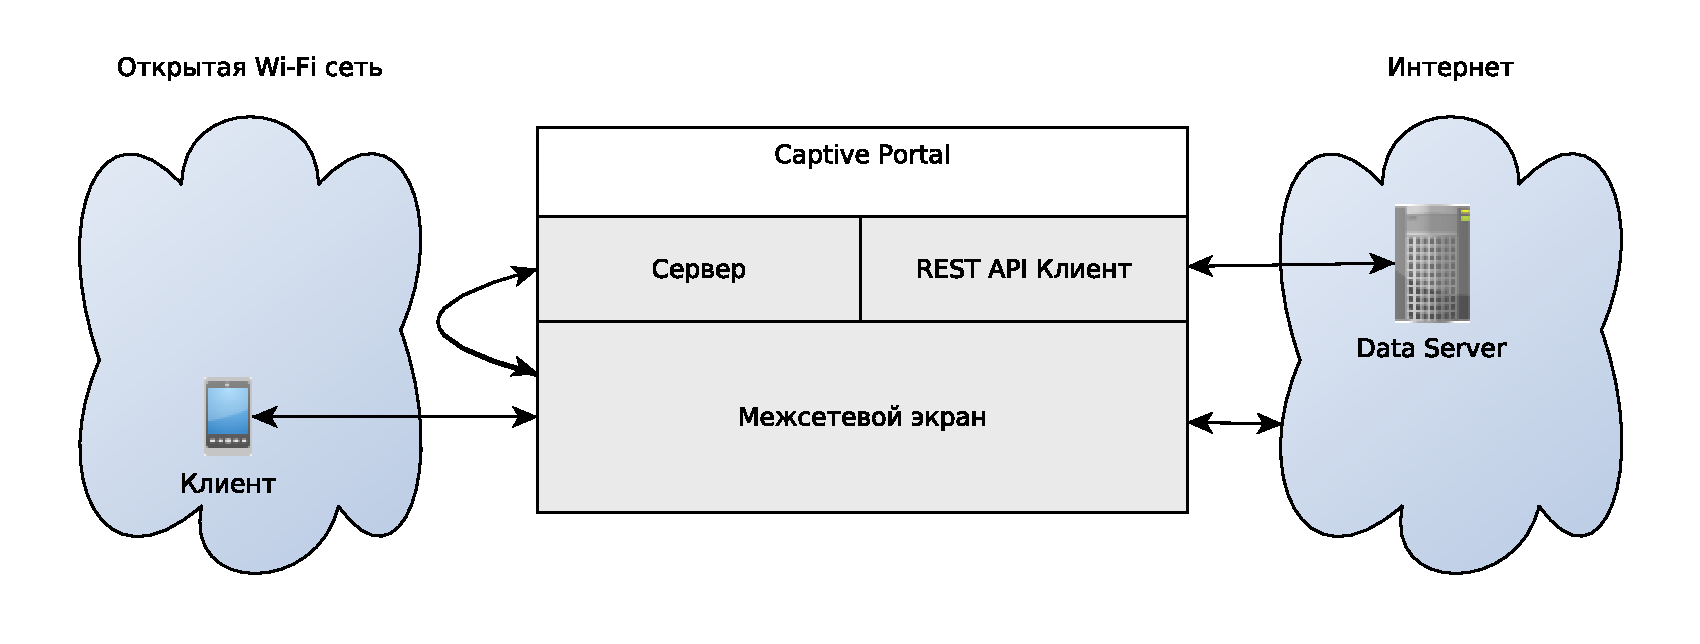
\includegraphics[width=\linewidth]{fig/CPArchitecture}
	\caption{Архитектура компонента регистрации}
	\label{fig:CPArchitecture}
\end{figure}

\textbf{Сервер} необходим для первоначального обслуживания клиентов. Данный модуль слушает 80 и 443 третий порты и работает по протоколу HTTP и HTTPS соответственно. В его задачи входит:

\begin{itemize}
	\item показ страницы регистрации;
	\item показ пользователького соглашения;
	\item получение регистрационных данных;
	\item формирование события регистрации клиента;
	\item формирование события, разрешающего клиенту доступ в интернет.
\end{itemize}

\textbf{REST API Клиент} позволяет проверять MAK адрес устройства клиента в базе системы. При наличие адреса, клиенту предоставляется доступ в интернет. Данный модуль также отвечает за регистрацию новых клиентов. Передача данных между модулем и сервером системы осуществляется по протоколу HTTPS, что позволяет защитить информацию от злоумышленников.

\textbf{Межсетевой экран} осуществляет следующие функции:
\begin{itemize}
	\item перенаправляет все запросы новых клиентов на сервер Captive Portal;
	\item блокирует доступ в интернет всем не авторизованым пользователям;
	\item предоставляет доступ в интернет клиентам по команде от сервера Captive Portal.
\end{itemize}

\subsection{Разработка компонента}

Для организации открытой Wi-Fi сети решено использовать утилиту hostapd[1]. Утилита позволяет создавать Wi-Fi точку доступа с различными настройками путем конфигурации фала настроек. Используемой в компоненте файл настроек представлен в листинге \ref{listings:hostapd}.

Для корректной работы Wi-Fi сети необходимо наличие DHCP сервера. Роль DHCP серврера в рассмотриваемом компоненте выполняет утилита dnsmasq. Для удобства обращение к серверу Captive Portal по установленному локальному имени (localcaptive) испольозуется DNS сервер, который также реализован в утилите dnsmasq. Конфигурационный файл dnsmasq представлен в листинге \ref{listings:dnsmasq}

Предполагается, что разрабатываемый программный компонент будет устанавливаться в устройства со слабой производительностью. К таким устройстам относятся большинство домашних роутеров. Ресурсы таких устройств сильно ограничены. Они могут иметь количество памяти до 20 мб и частоту одноядерного процессора до 500 MHz. В таких условиях использование таких утилит как apache и nginx существенно замедлит работу устройства. В связи с этим, принято решение разрабатывать свой сервер на языке C++.

Для ускорения разработки и уменьшения количества ошибок было решено использовать заготовку для веб-сервера[2], написанную на языке С++ и распространяемую по лицензии MIT[3]. В своей работе данная закотовка использует библиотеку boost.asio[4], которая позволяет при необходимости вносить изменения в исходный код как сервера так и библиотеки.

На рисунке \ref{fig:CPUML} представлена UML диаграмма компонента регистрации

\begin{figure}[H]
	\centering
	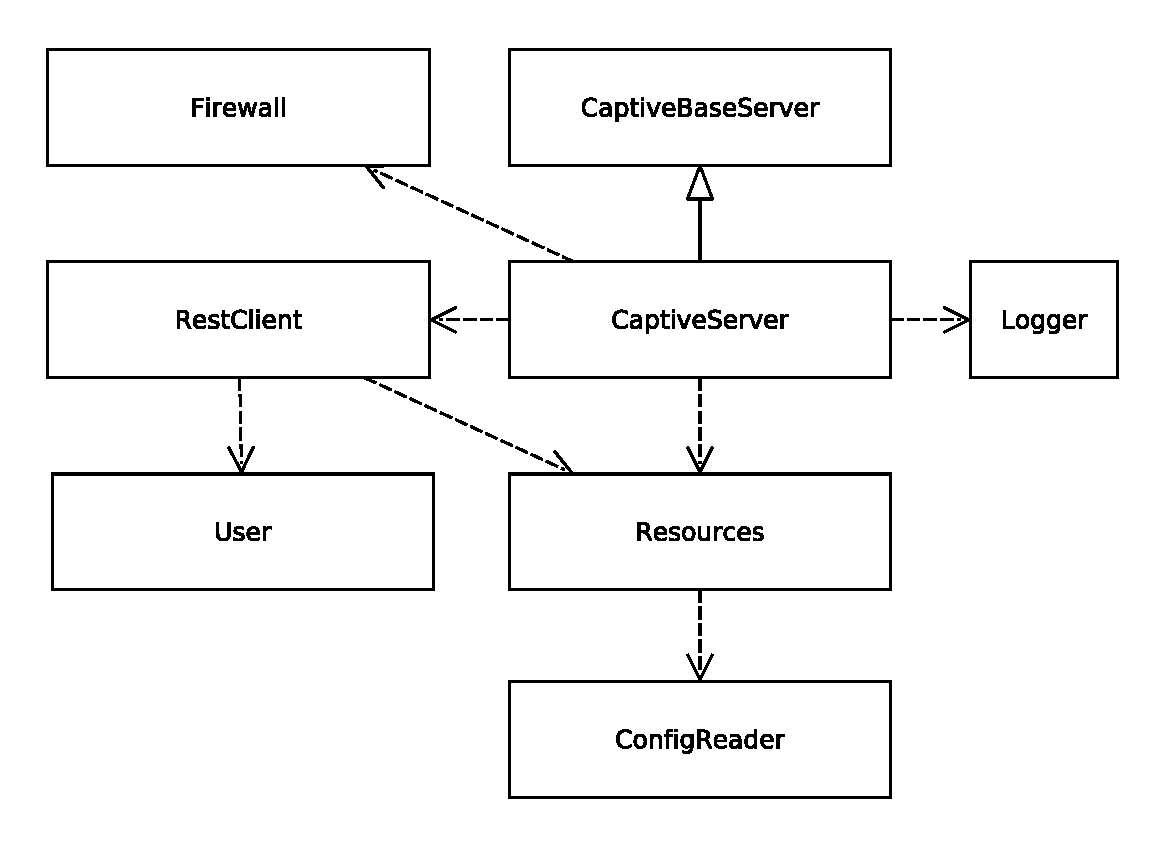
\includegraphics[width=\linewidth]{fig/CPUML}
	\caption{UML диаграмма компонента регистрации}
	\label{fig:CPUML}
\end{figure}

Рассмотрим кадый класс и наиболее значимые методы по отдельности.

\textbf{CaptiveBaseServer.}
\textbf{CaptiveServer.}
Функцией этого класса является поддержание работоспособности сервера и выдача команд межсетевому экрану и REST API слиенту.

\textbf{Firewall.}

Объект этого класса выполняет функции сетевого экрана, позволяющие блокировать клиентам доступ в интернет до момента получения команды из класса CaptiveServer.

\textbf{RestClient.}

Данный класс регистрирует на сервре новых клиентов и проверяет наличие MAC адреса в базе данных сервера таргетированной рекламы.

Метод \textit{bool RestClient::isClientExist(std::string mac)} получает в качестве параметра MAC адрес устройства клиента в виде AA:BB:CC:DD:EE:FF. Его задача установить зарегистрирован ли данный MAC в системе. Возвращаемое значение равно true елсли адрес уже существует. В противном случае возвращается false.

Метод \textit{bool RestClient::registerClient(User user)} получает в качестве параметра объект класса User и совершает попытку его регистрации на сервере. В случае успеха возращается true, иначе false.

\textbf{User.}

Отвечает за данные, полученные от клиента при регистрации. Поля данного класса отправляются на сервер для регистрации нового клиента.

\textbf{Resources.}

Класс, реализующий паттерн проектирования Singleton. Единственный экземпляр этого класса содержит информацию о всех ресурсах, записанных в конфигурационном файле и необходимых в других компонентах системы.

\textbf{ConfigReader.}

Объект этого класса позволяет считывать конфигурационный файл, сформированный по правилу <<ресурс = значение>>.

\textbf{Logger.}

Еще один класс, реализующий паттерн проектирования Singleton. Позволяет вести логирование работы системы. Логируемые сообщения имеют один из четырех уровней, определенных в перечислении LogLevel: ERROR, WARNING, INFO, DEBUG.

Метод \textit{Logger::get(LogLevel level)} возращает единственный экземпляр класса Logger и задает уровень логирования.

Для объектов класса переопределен оператор <<<<>>, что позволяет использовать класс следующим образом:

Logger::get(LogLevel::INFO) << System started << std::endl;

Метод \textit{std::string Logger::getTimeForFileName()} позволяет получить время, сформированное в имени файла логов.

Метод \textit{std::string Logger::getTimeForFileName()} возвращает время, вставляемое перед каждым сообщением при логировании. Пример файла с логами представлен в листинге \ref{listings:CPlog}

%%%%%%%%%%%%%%%%%%%%%%%%%%%%%%%%%%%%%%%%%%%%%%%%%%%%%%%%%%%%%%%%%%%%%%%%%%%%%%%%
\section{Проектирование и разработка Wi-fi сканера}
%%%%%%%%%%%%%%%%%%%%%%%%%%%%%%%%%%%%%%%%%%%%%%%%%%%%%%%%%%%%%%%%%%%%%%%%%%%%%%%%

В список задач Wi-Fi сканера входят:

\begin{itemize}
	\item мониторин радиоканала на частоте 2.4 ГГц;
	\item определение новых устройств в радиусе досягаемости Wi-Fi модуля;
	\item регистрация MAC-адреса устройства на сервере таргетированной рекламы.
\end{itemize}

\subsection{Проектирование архитектуры}

Архитектура Wi-Fi сканера состоит из двух модулей: сканера Wi-Fi сети и модуля регистрации посеещений. На рисунке \ref{fig:WiFiScanerArch} представлена архитектура Wi-Fi сканера.

\begin{figure}[H]
	\centering
	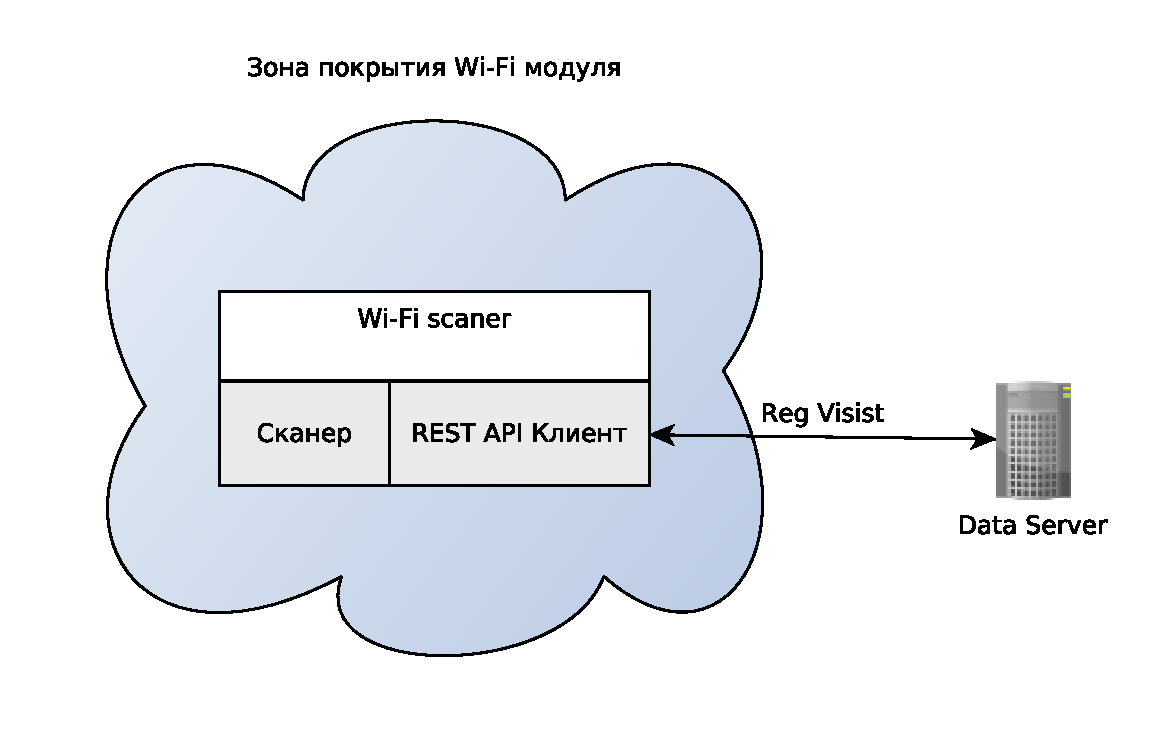
\includegraphics[width=\linewidth]{fig/WiFiScanerArch}
	\caption{Архитектура Wi-Fi сканера}
	\label{fig:WiFiScanerArch}
\end{figure}

\textbf{Сканер} осуществляет мониторинг пакетов стандарта 802.11. При выявлении пакетов от нового клиента MAC-адрес устройства отправителя сохранятеся в память для дальнейшей обработки.

\textbf{REST API клиент} регистрирует новые устройства на сервере таргетированной рекламы.

\subsection{Разработка компонента}

Wi-Fi монитор, как и компонент регистрации должен работать на устройстве со слабой производительностью. Из этого следует, что рассмтриваемый компонент также будет реализован на языке C++. Для реализации функциональности монитора решено использовать библиотеку pcap[5]. Библиотека позволяет задавать необходимые настройка интернет адаптеру и просматривать все полученные им пакеты. pcap используют в своей работе такие программы как Wireshark и tcpdump. Для успешного захвата всех пакетов Wi-Fi модулем, необходимо предварительно перевести его в режим монитора. Библиотека pcap позволяет легко сделать это.

% [1] https://w1.fi/hostapd/
% [2] https://github.com/eidheim/Simple-Web-Server
% [3] https://github.com/eidheim/Simple-Web-Server/blob/master/LICENSE
% [4] https://www.boost.org/doc/libs/1_66_0/doc/html/boost_asio.html
% [5] https://www.tcpdump.org/manpages/pcap.3pcap.html